\subsection{Probability and Combinatorics}

\subsubsection{Probability}
Probability is the likelihood of an event occurring. (the number of possibilities that satisfy a given constraint over the number of possible outcomes)\\
Probability is always expressed as a number between $0$ and $1$.\\
The probability of an event, $A$, is denoted by $P(A)$.\\
The sum of all possibilities of an event is equal to $1$.\\
Relative frequency is the frequency of an event occurring in a trial to provide an estimate of the probability. Note that the more trials, the better the estimate will be.\\
\\
Definitions:
\begin{itemize}
    \item Two events are mutually exclusive if they cannot occur at the same time.
    \item The probability of event $A$, given event $B$, is called conditional probability. $P(A|B)$ is conditional probability of $A$, given $B$.
    \item The intersection of two events is the likelihood of both events occurring. It is the set of elements that are common to both events. Denoted by $P(A\cap B)$
    \item The union of two events is the probability of at least one of the events occurring. Denoted by $P(A\cup B)$
    \item Independent Events: The probability of $A$ does not affect the probability of $B$.
    \item Dependent Events: Occurrence of event $A$ changes the probability of event $B$ occurring.
    \item The compliment of an event is the case of an event not occurring. $P(A')$ is the probability that $A$ does not occur.
\end{itemize}
Rules of Probability:
\begin{align*}
    &P(A)+P(A')=1\\
    &P(A\cap B)=P(A)P(B|A)\\
    &P(A\cup B)=P(A)+P(B)-P(A\cap B)
\end{align*}

\subsubsection{Combinatorics}
Consider a task made up of several stages. The number of choices for the first stage is $a$, the number for the second stage is $b$, then $c$ and so on. The number of ways the task can be completed (or the number of possible outcomes) is: $a\cdot b\cdot c\cdot d\cdots$\\
Ex: using the letters $A, B, C,D,E,F$, how many 4 letter combinations can be made if:\\
a) letters can be repeated?\\
b) letters can not be repeated?\\
a) $6\cdot6\cdot6\cdot6=6^4=1296$\\
b) $6\cdot5\cdot4\cdot3=360$\\
\\
Factorial Notation:\\
The symbol '!' indicates factorial and means the product of decreasing natural numbers
$$n!=n(n-1)(n-2)\cdots3\cdot2\cdot1=\prod_{i=1}^ni$$
Ex: Simplify $\dfrac{25!}{23!5!}$
\begin{align*}
    \frac{25\cdot24\cdot23!}{23!5\cdot4\cdot3\cdot2\cdot1}=\frac{25\cdot24}{5\cdot4\cdot3\cdot2}=5
\end{align*}
Ex2: Simplify $\dfrac{(n+1)!}{(n-1)!}$
\begin{align*}
    \frac{n+1)(n)(n-1)!}{(n-1)!}=n(n+1)
\end{align*}
\\
Permutations:\\
A permutation is an arrangement of distinct objects in which the order is important.\\
The number of permutations of $n$ distinct objects is $n!$\\
The number of permutations of $n$ distinct objects taken $r$ at a time is:
$$\prescript{}{n}{P}_r=\frac{n!}{(n-r)!}$$
Ex: licence plates have 3 digits followed by 3 letters. How many different plates can be made?\\
\begin{align*}
    \perm{10}{3}\perm{26}{3}=\frac{10!}{(10-3)!}\frac{26!}{(26-3)!}=11232000
\end{align*}
Ex2: Solve for $n$ if $\perm{n}{2}=30$
\begin{align*}
    &\frac{n!}{(n-2)!}=30\\
    &\frac{n(n-1)(n-2)!}{(n-2)!}=30\\
    &n^2-n=30\\
    &n^2-n-30=0\\
    &(n-6)(n+5)=0\\
    &\Ra n=6,\,n=-5\\
    &n\neq-5\text{ because }n\in\mathbb{N}\\
    &\therefore n=6
\end{align*}
Some permutations have restrictions where certain objects must be grouped. If objects are grouped together, the number of possible outcomes can be calculated by multiplying:\\
(total number of groups or individuals)!(number in group 1)!(number in group 2)!$\cdots$\\
Ex: How many ways can "PICTURE" be arranged if:\\
a) two vowels must be together?\\
b) A vowel cannot be beside another vowel?\\
\\
a) This forms 6 groups with one group of two so $6!2!=1440$\\
b) For this one we can calculate it by taking the total arrangements, $7!$, and subtracting the arrangements that don't fit the criteria.\\
3 vowels together: $5!3!$\\
2 vowels together: $6!2!$\\
So the answer will be: $7!-5!3!-6!2!=280$\\
\\
If there are repetitions, the number of permutations can be expressed as $\dfrac{n!}{a!b!c!\cdots}$ where $a$, $b$, and $c$ are the number of repetitions for each identical object\\
Ex: a true-false quiz has 10 questions. How many answer keys are possible if 4 are true and 6 are false?\\
$\dfrac{10!}{6!4!}=210$\\
\\
Combinations:\\
A combination is an arrangement of distinct objects in which the order of the objects is not important.
$$\comb{n}{r}=\frac{\perm{n}{r}}{r!}=\frac{n!}{r!(n-r)!}=\left(\begin{matrix} n\\r\end{matrix}\right)$$
Ex: Looking at a 5-card hand in a deck of cards:\\
a) how many 5 card hands are there?\\
b) how many with all hearts?\\
c) how many with 3 hearts and 2 spades?\\
d) how many with at most 3 hearts?\\
\\
a) $\comb{52}{5}=2598960$\\
b) $\comb{13}{5}\comb{39}{0}=1287$\\
c) $\comb{13}{3}\comb{13}{2}\comb{39}{0}$\\
d) We can sum all the different possibilities
\begin{align*}
    &\text{3 hearts: }\comb{13}{3}\comb{39}{2}\\
    &\text{2 hearts: } \comb{13}{2}\comb{39}{3}\\
    &\text{1 heart: }\comb{13}{1}\comb{39}{4}\\
    &\text{0 hearts: }\comb{13}{0}\comb{39}{5}\\
    &\text{Total is }2569788
\end{align*}

\subsubsection{Pascal's Triangle}
\centerline{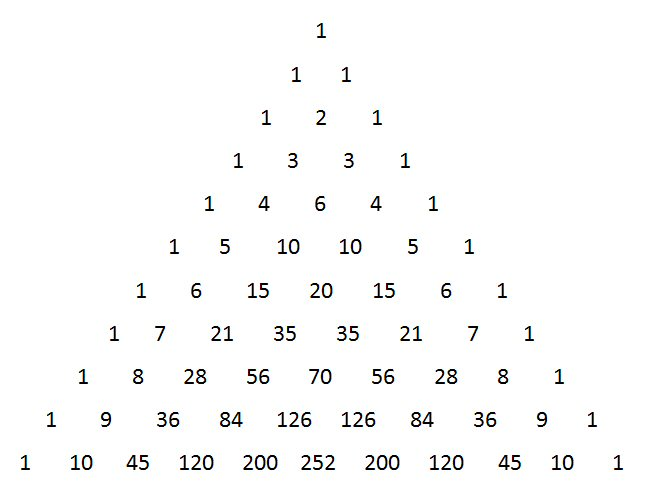
\includegraphics[scale=0.5]{Images/FundamentalsPictures/PascalTriangle.jpg}}
It can also be written using combinations for where $n$ is the row number and $r$ is the term number where we start counting from 0.\\
\centerline{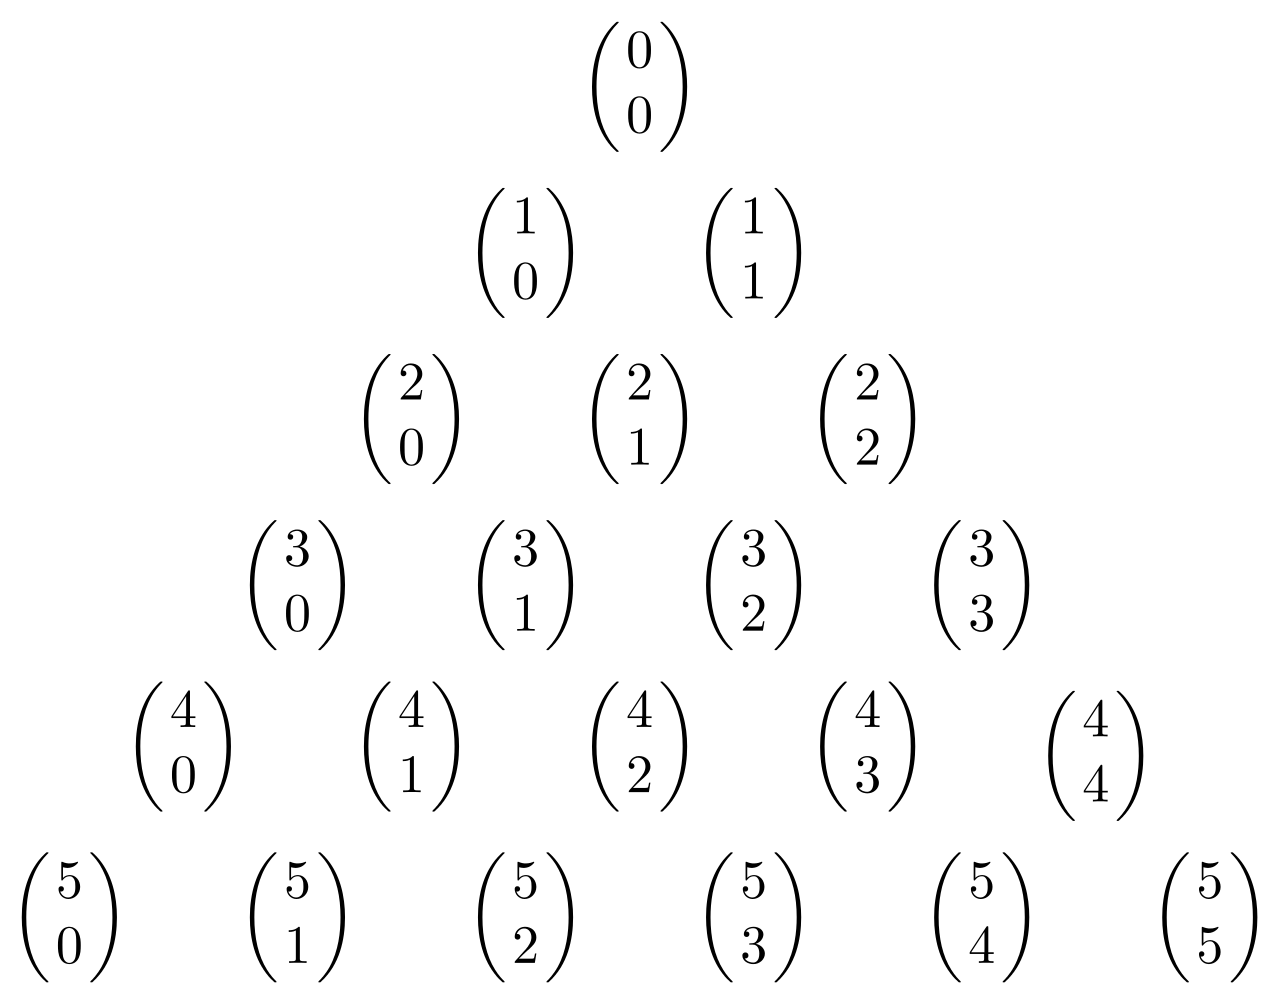
\includegraphics[scale=0.2]{Images/FundamentalsPictures/PascalTriangleComb.png}}\\
The sum of each row can be expresses by the geometric sequence $t_n=2^{n-1}$ where $n$ is the row number and $t_n$ is the sum of that row.\\
\\
Pathway Problems:\\
Another occurrence of Pascal's triangle is if we want to find the number of different possible pathways to travel to a point on a grid.\\
\centerline{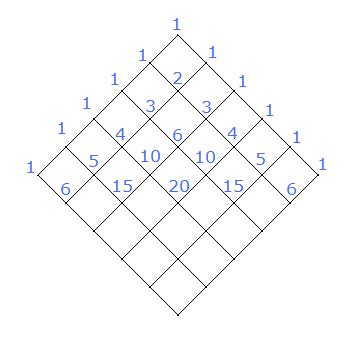
\includegraphics[scale=0.55]{Images/FundamentalsPictures/PascalTrianglePathway.png}}
For a simple grid as shown, we can find the number of pathways using permutations.\\
For the 5x5 grid, we go down 5 moves and right 5 moves for a total of 10 moves. So we can express it as $\dfrac{10!}{5!5!}=252$ moves.\\
Note that this only works for perfect grids. A more difficult example, we need to use the general process of Pascal's triangle and sum adjacent corners to come to the answer.\\
Ex:\\
\centerline{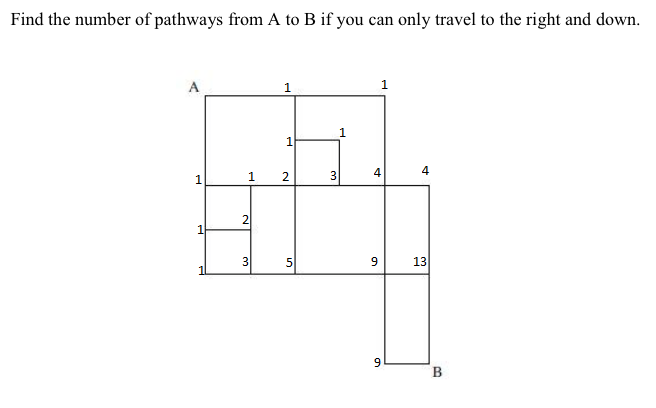
\includegraphics[scale=0.8]{Images/FundamentalsPictures/PathwayEx.png}}
So there will be a total of 22 different paths between A and B.\\
\\
The Binomial Theorem:\\
This is used to expand any power of a binomial expression $(a+b)^n$\\
It follows the patterns of Pascal's triangle and can be expressed as:
$$(a+b)^n=\comb{n}{0}(a)^n(b)^0+\comb{n}{1}(a)^{n-1}(b)^1+\comb{n}{2}(a)^{n-2}(b)^2+\cdots+\comb{n}{n-1}(a)^1(b)^{n-1}+\comb{n}{n}(a)^0(b)^n$$
$$(a+b)^n=\sum_{k=0}^n\left(\begin{matrix}n\\k\end{matrix}\right)a^{n-k}b^k$$

